% !TEX root = ../literature.tex
\subsection{Discussion}
%this section needs to be called discussion, and you need to use it to discuss a bit more about the relationships between the different fields, concluding with the idea that some sharing of information across these areas to futher research various aspects would be a good idea. So you are on the right track - but you need to be a bit more detailed in your thinking

The current paper aims to analytically summarize published research within e preset interest area. In the current section we would expand on the relationships between presented different fields, we believe this will further deepen our understanding of them.\\
%The findings of this work are that gesture recogntion using touchscreens is now a mature enough technology that it is ready for implementation in commerical products. The iPhone has shown that basic gesturing has a place in mobile operating systems and my results show that more complex gestures can be easily recognised and recognised accurately. The problem is context.
Many researchers had spent time and effort to explore how large displays aid in improving people's experiences. 
With the shift from private to public settings the explored solutions changed. 
It was highly impractical to put wires on people who wanted to use an installation naturally in a public environment [9].\\

With this limitation came different approaches for solving it. 
We identified two different areas which deals with it, we present them in \Cref{fig:litreview}.

\begin{figure}[h!]
\centering
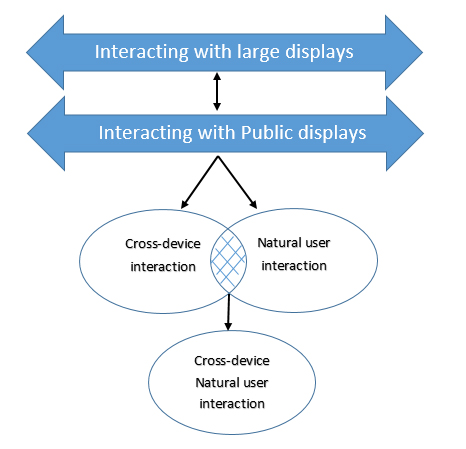
\epsfig{file=images/litreview-fig1.jpg, width=0.5\textwidth}
\caption{Write Caption}
\label{fig:litreview}
\end{figure}

The fields of natural user interactions and cross-device interactions were thoroughly examined. 
We were surprised to see that research in combining features from the two areas is slim even though they are complementary to each other. 
There was research that was done [26, 27, 28, 29]. 
Interaction-techniques were evaluated with 3-6 people using qualitative surveys in [27,28,29] and without qualitative surveys in [26].\\

In summary, we can see research opportunities in further exploration of cross-device natural user interactions technique for large displays. We believe the limitations that each of these fields ignore is the interaction space between them. To move beyond this limitation, we believe a unification of these discrete interaction techniques in continuous interaction space and it's further research would be positive and beneficial.
Firstly, as handheld devices become thinner and lighter and spatially-aware technologies, such as Kinect, continue to evolve, this opens a potentially rich space of aforementioned techniques. 
Secondly, we see opportunities in quantitative aspect, for example comparative study of different interaction techniques. 
